\documentclass[../Main.tex]{subfiles}

\begin{document}

\section{Design und Umsetzung des Kampfabschnitts} \label{sec:Umsetzung}

In diesem Kapitel werden zunächst Designvorschläge für die beiden inhaltlichen Komponenten der Erkenntnisfrage (Abschnitt~\ref{sec:Erkenntnisfrage}) aufgestellt: Gegnerverhalten und Kampfgefühl einerseits, Gegnerplatzierung und Leveldesign andererseits. Sie zielen auf die drei dort genannten spielerischen Qualitäten ab, nämlich einen nachvollziehbaren Spielfluss, eine angemessene Schwierigkeit und ein befriedigendes Spielgefühl. Dazu werden die Erkenntnisse aus der Referenzspielanalyse (Kapitel~\ref{sec:Referenzspielanalyse}) und der Leveldesign-Recherche (Kapitel~\ref{sec:Leveldesign}) zu spezifischen Designvorschlägen für unseren Kampfabschnitt verdichtet. Es konnten nicht alle Recherchepunkte in den Designvorschlägen verwertet werden, da es uns im vorgegebenen Zeitraum nicht möglich war. Deshalb haben wir die Punkte Rausgesucht, die wir als besonders wichtig für unsere Leitfrage oder als überprüfbar eingeschätzt haben. Anschliessend wird für jeden Vorschlag beschrieben, wie er im Prototyp umgesetzt wurde und wo sich die Umsetzung überprüfen lässt. Die Überprüfung mittels Playtests folgt in Kapitel~\ref{sec:Evaluation}.

\subsection{Von der Recherche zu den Designvorschlägen} \label{sec:Designvorschlaege}

Jeder Designvorschlag folgt demselben Schema: der Vorschlag selbst, sein Nutzen, also welcher Aspekt der Erkenntnisfrage damit bedient wird, und die Herleitung aus Recherche und Spielanalysen.

\begin{table}[H]
    \centering
    \small
    \renewcommand{\arraystretch}{1.3}
    \begin{tabular}{|>{\raggedright\arraybackslash}p{0.6cm}|>{\raggedright\arraybackslash}p{4.3cm}|>{\raggedright\arraybackslash}p{6.6cm}|>{\raggedright\arraybackslash}p{1.8cm}|}
        \hline
        \textbf{Nr.} & \textbf{Designvorschlag} & \textbf{Herleitung} & \textbf{Playtest} \\
        \hline
        \multicolumn{4}{|l|}{\textit{Gegnerverhalten (Abschnitt~\ref{sec:UmsetzungGegner})}} \\
        \hline
        V1 & Überlegenheit als Grundzustand & Kontrast \game{NieR: Automata} / \game{Ninja Gaiden} (Abschnitte~\ref{sec:ReferenzspielanalyseNier} und~\ref{sec:ReferenzspielanalyseNinja}); emotionsgeleitetes Design (Abschnitt~\ref{sec:Pacing}) & Q1, B1 \\
        \hline
        V2 & Begrenzung gleichzeitiger Angreifer & Beide Referenzspiele (Abschnitt~\ref{sec:Vergleich}); Pacing (Abschnitt~\ref{sec:Pacing}) & Q2, B2 \\
        \hline
        V3 & Taktisches Dilemma durch zwei Gegnerrollen & Frage D2 beider Analysen; Gegnerrollen im Encounter-Design (Abschnitt~\ref{sec:Encounter}) & Q3, B3 \\
        \hline
        V4 & Klar telegrafierte Angriffe & \game{NieR: Automata}, Frage M2; Lesbarkeit (Abschnitt~\ref{sec:Encounter}) & Q4, B4 \\
        \hline
        \multicolumn{4}{|l|}{\textit{Gegnerplatzierung und Kampfraum (Abschnitt~\ref{sec:UmsetzungLevel})}} \\
        \hline
        V5 & Lesbare Platzierung, dynamisches Verhalten & \game{NieR: Automata}, Frage A3; \game{Ninja Gaiden}, Frage D3 (Abschnitt~\ref{sec:Vergleich}); Lesbarkeit (Abschnitt~\ref{sec:Encounter}) & Q5, B6 \\
        \hline
        V6 & Der Raum als Druckmittel & \game{Ninja Gaiden}, Frage M3; räumliche Typologien (Abschnitt~\ref{sec:Raumtypologien}) & Q6, B7 \\
        \hline
        V7 & Wellenstruktur mit Erholungsphasen & \game{Ninja Gaiden}, Frage D1; \game{NieR: Automata}, Frage A4; Rollercoaster-Pacing (Abschnitt~\ref{sec:Pacing}) & Q7, B8 \\
        \hline
        V8 & Gestaffelte Einführung neuer Gegner & Scaffolding (Abschnitt~\ref{sec:Scaffolding}); \game{NieR: Automata}, Frage D1 & Q8, B9 \\
        \hline
    \end{tabular}
    \caption{Übersicht der Designvorschläge mit Herleitung und zugehörigen Playtest-Items}
    \label{tab:Designvorschlaege}
\end{table}

\begin{itemize}[leftmargin=1.5cm]
    \item \textcolor{red}{Tabelle prüfen und ggf. ergänzen; die Items Q9--Q11 sowie B5 und B10--B14 betreffen den gesamten Kampfabschnitt und keinen einzelnen Vorschlag.}
    \item \textcolor{red}{Optional: kurzer Satz, warum gerade diese acht Vorschläge ausgewählt wurden und was bewusst nicht umgesetzt wurde (z.\,B. Elemente aus den Analysen, die verworfen wurden, und weshalb).}
\end{itemize}

\subsection{Gegnerverhalten und Spieler-Gegner-Interaktion} \label{sec:UmsetzungGegner}

\subsubsection{Überblick über die Gegnertypen} \label{sec:Gegnertypen}

In unserem Prototyp gibt es zwei Gegnerklassen, Nah- und Fernkämpfer, von denen es jeweils mehrere Varianten gibt: zwei Nahkämpfer und drei Fernkämpfer. Insgesamt gibt es damit fünf verschiedene Gegnertypen (Abbildung~\ref{fig:Gegnertypen}). Farblich sind die Nahkämpfer rötlich und die Fernkämpfer gelblich gehalten.

\begin{figure}[H]
    \centering
    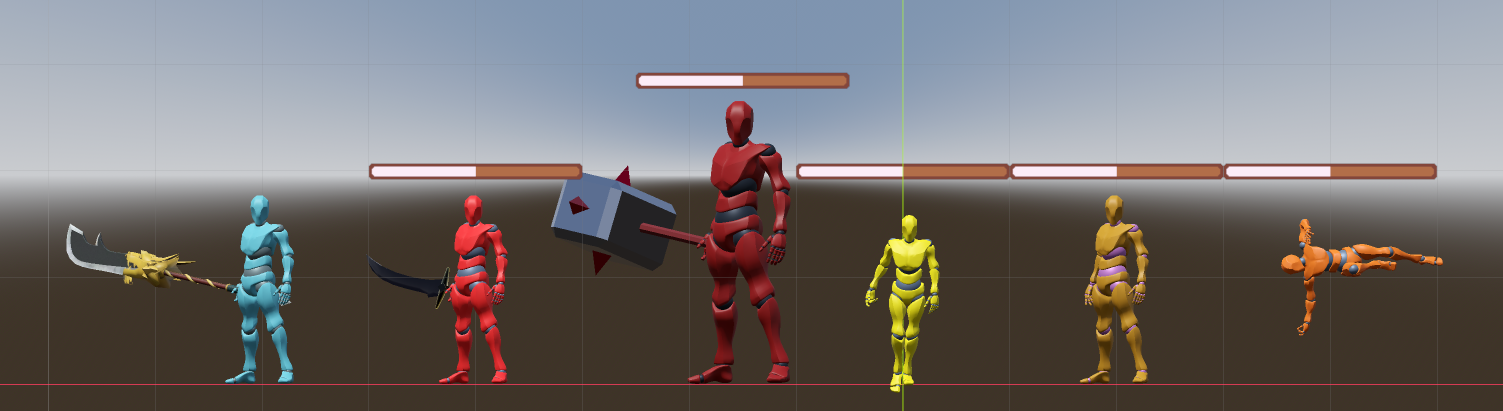
\includegraphics[width =\linewidth]{Assets/All Entities.png}
    \caption[Die fünf Gegnertypen des Prototyps. Eigene Abbildung.]{Die fünf Gegnertypen des Prototyps und der Spieler, von links nach rechts: Spieler (Blau), Soldier (Rot), Heavy Soldier (Dunkelrot), Archer (Gelb), Heavy Archer (Hellbraun), Chain Archer (Orange). Eigene Abbildung.}
    \label{fig:Gegnertypen}
\end{figure}

Der Soldier ist der grundlegende Nahkämpfer, der auf den Spieler zurennt und zuschlägt. Der Heavy Soldier ist grösser, stärker und langsamer als der Soldier und hat mehr Lebenspunkte, zeigt aber dasselbe Verhalten.

Die Fernkämpfer bewegen sich alle nicht. Der Archer schiesst ein Projektil auf den Spieler. Der Heavy Archer macht dasselbe, sein Projektil ist jedoch langsamer, kann dafür die Richtung ändern und verfolgt den Spieler. Der Chain Archer schiesst gleich drei Pfeile auf den Spieler, die mehr als doppelt so schnell sind wie jene des Archers.

Die Reichweite der Archers ist gleich, also die Distanz von der aus sie auf den Spieler Schiessen können. Lebenspunkte und Schaden unterscheiden sich dagegen je nach Gegnertyp; Tabelle~\ref{tab:Gegnertypen} fasst die Eigenschaften zusammen.

\begin{table}[H]
    \centering
    \small
    \renewcommand{\arraystretch}{1.3}
    \begin{tabular}{|>{\raggedright\arraybackslash}p{2.3cm}|>{\raggedright\arraybackslash}p{2.9cm}|>{\raggedright\arraybackslash}p{3.0cm}|>{\raggedright\arraybackslash}p{0.8cm}|>{\raggedright\arraybackslash}p{1.4cm}|>{\raggedright\arraybackslash}p{1.9cm}|}
        \hline
        \textbf{Gegnertyp} & \textbf{Bewegung} & \textbf{Angriff} & \textbf{LP} & \textbf{Schaden} & \textbf{Unter\-brechbar} \\
        \hline
        \multicolumn{6}{|l|}{\textit{Nahkämpfer (rötlich)}} \\
        \hline
        Soldier & rennt auf den Spieler zu & Nahkampfschlag & 130 & 15 & ja \\
        \hline
        Heavy Soldier & wie Soldier, aber langsamer; grösser & wie Soldier & 200 & 30 & nein \\
        \hline
        \multicolumn{6}{|l|}{\textit{Fernkämpfer (gelblich)}} \\
        \hline
        Archer & stationär & ein Projektil & 60 & 10 & ja \\
        \hline
        Heavy Archer & stationär & ein langsameres, zielsuchendes Projektil & 40 & 20 & ja \\
        \hline
        Chain Archer & stationär & drei Pfeile, mehr als doppelt so schnell wie beim Archer & 70 & $3 \times 10$ & ja \\
        \hline
    \end{tabular}
    \caption{Eigenschaften der fünf Gegnertypen (LP = Lebenspunkte)}
    \label{tab:Gegnertypen}
\end{table}

\paragraph{Abstimmung von Schaden und Lebenspunkten}
Der Spieler selbst hat 200 Lebenspunkte. Seine Angriffe verursachen je nach Combo unterschiedlich viel Schaden (Tabelle~\ref{tab:Combos}).

\begin{table}[H]
    \centering
    \small
    \renewcommand{\arraystretch}{1.3}
    \begin{tabular}{|l|l|l|}
        \hline
        \textbf{Combo} & \textbf{Schaden pro Treffer} & \textbf{Gesamt} \\
        \hline
        Light Combo & 20, 20, 30, 40 & 110 \\
        \hline
        Heavy Combo & 30, 30, 40 & 100 \\
        \hline
        Air Combo & 20, 20, 20, 20 & 80 \\
        \hline
    \end{tabular}
    \caption{Schaden der Combos des Spielers}
    \label{tab:Combos}
\end{table}

Die Schadenswerte und Lebenspunkte wurden so gewählt, dass bestimmte Combos einen Gegner genau mit dem letzten Schlag besiegen, weil wir davon ausgingen, dass sich dies besser anfühlt: Eine Heavy Combo besiegt einen Chain Archer mit ihrem letzten Schlag, und der Heavy Soldier stirbt nach genau zwei Heavy Combos. Gleichzeitig haben wir darauf geachtet, dass zum Beispiel ein Soldier eine Light Combo knapp überlebt. Dadurch entsteht beim Spielen Variation, und der Spieler muss Combos abbrechen oder kombinieren.

\begin{itemize}[leftmargin=1.5cm]
    \item \textcolor{red}{Bild einfügen (Platzhalter in Abbildung~\ref{fig:Gegnertypen}).}
    \item \textcolor{red}{Schreibweise: im Text jetzt einheitlich \enquote{Soldier} (vorher teils \enquote{Solider}). Prüfen, ob die Codenamen im Spiel genauso heissen, und überall gleich verwenden (auch im Anhang).}
    \item \textcolor{red}{\enquote{Die Reichweite der Gegner ist gleich}: gilt das für alle fünf Typen, also auch für die Fernkämpfer? Präzisieren, wenn möglich mit Werten.}
    \item \textcolor{red}{Spalte \enquote{Unterbrechbar} stammt aus eurem Text in V1 (\enquote{alle ausser dem Heavy Soldier}) -- bitte prüfen, ob das auch für die Archers stimmt.}
    \item \textcolor{red}{Optional: Bewegungs- und Projektilgeschwindigkeiten als Werte ergänzen.}
    \item \textcolor{red}{\enquote{weil wir davon ausgingen, dass sich dies besser anfühlt} ist eine Hypothese -- im Playtest bestätigt? Ggf. in Kapitel~\ref{sec:Evaluation} aufgreifen.}
    \item \textcolor{red}{Gemeinsame Basisklasse und Verhaltensarchitektur kurz nennen (Rückbezug auf Abschnitt~\ref{sec:Kernmechanik}); Details mit konkretem Verweis auf die technische Dokumentation.}
\end{itemize}

\subsubsection{V1: Überlegenheit als Grundzustand} \label{sec:V1}

\paragraph{Vorschlag und Herleitung}
Der Spieler soll sich seinen Gegnern grundsätzlich überlegen fühlen, wobei dieser Zustand gezielt durchbrochen werden kann. Der Nutzen liegt im Spielgefühl: Aggression soll sich sicher und belohnt anfühlen, während Spannung erst dort entsteht, wo die Kontrolle kurzzeitig bedroht wird. Hergeleitet ist der Vorschlag aus dem Kontrast der beiden Referenzspiele, der dauerhaften Überlegenheit in \game{NieR: Automata} (Abschnitt~\ref{sec:ReferenzspielanalyseNier}) gegenüber dem prekären Gleichgewicht in \game{Ninja Gaiden} (Abschnitt~\ref{sec:ReferenzspielanalyseNinja}), sowie aus dem Prinzip des emotionsgeleiteten Designs (Abschnitt~\ref{sec:Pacing}).

\paragraph{Umsetzung im Prototyp}
Im Eins-gegen-eins ist der Spieler jedem einzelnen Gegner haushoch überlegen. Er verursacht meist doppelt bis viermal so viel Schaden wie die Gegner und hat auch doppelt bis viermal so viele Lebenspunkte, mit Ausnahme des Heavy Soldiers, der mit 200 Lebenspunkten genau gleich viele hat (Tabelle~\ref{tab:Gegnertypen}). Zudem hat jeder Gegner ein simples Moveset, also nur eine begrenzte Anzahl Bewegungen, die er ausführen kann. Der Spieler hat deutlich mehr: Er kann zum Beispiel schneller rennen, springen, was keiner der Gegner kann, und sich sogar heilen. Ausserdem sind alle Gegner ausser dem Heavy Soldier unterbrechbar, was sie im direkten Nahkampf sehr schwach macht.

Man könnte deshalb annehmen, dass der Spieler auch grosse Mengen von Gegnern problemlos bewältigt. Das stimmt allerdings nicht ganz, denn die Überlegenheit wird an mehreren Stellen gezielt durchbrochen:

\begin{itemize}[leftmargin=1.5cm]
    \item In der Gruppe stimmen sich die Gegner miteinander ab und stellen so eine grössere Gefahr dar (Abschnitte~\ref{sec:V2} und~\ref{sec:V3}).
    \item Einige Gegner lassen sich nicht mit einer einzigen Combo besiegen, was grosse Horden zusätzlich gefährlich macht.
    \item Am Ende einer Combo weist der Spieler eine gewisse Trägheit auf. Wird der Gegner mit der Combo nicht besiegt, erhält dieser dadurch die Möglichkeit, den Spieler zu treffen.
    \item Das Heilen dauert eine gewisse Zeit. Gibt es zu wenig Platz und keine Möglichkeit, sich zu verstecken, ist es sehr schwer, sich zu heilen (vgl. Abschnitt~\ref{sec:V6}).
\end{itemize}

Als Alternative haben wir versucht, die Encounters durch mehr Lebenspunkte der Gegner sowie durch mehr und längere Wellen schwieriger zu machen. Wir haben uns aber gegen diese Lösungen entschieden, da sie das Spiel nur sinnlos strecken und keinen Mehrwert bieten. Zudem verlangsamen sie den Spielfluss, der nach unserer Vorstellung schnell und aggressiv sein soll (Abschnitt~\ref{sec:Genredefinition}). Der Spieler heilt jedes mal 50 Lebenspunkte auf einmal. mit einer vollen Manaleiste kann der spieler genau 200 Lebenspunkte heilen, also einmal von 0 auf 200 Lebenspunkte.

\begin{itemize}[leftmargin=1.5cm]
    \item \textcolor{red}{Faktoren prüfen: Laut Tabelle hat der Spieler gegenüber dem Soldier nur ca.\ 1,5-mal so viele LP (200 vs.\ 130), gegenüber dem Heavy Archer 5-mal (200 vs.\ 40). Beim Schaden (Spieler 20--40 pro Treffer) liegt der Heavy Soldier mit 30 ungefähr gleichauf. \enquote{Doppelt bis viermal} entsprechend anpassen oder genauer formulieren.}
    \item \textcolor{red}{Widerspruch: Hier steht, dass keiner der Gegner springen kann, in Raum~4 (Tabelle~\ref{tab:Raeume}) gibt es aber einen Soldier mit Sprungangriff. Klären (z.\,B. Angriff von erhöhter Position?).}
    \item \textcolor{red}{\enquote{stimmen sich miteinander ab}: kurz sagen, was genau gemeint ist (Angriffs-/Abstandsmodus aus V2?).}
    \item \textcolor{red}{Optional: Dauer der Trägheit am Combo-Ende und der Heilung als Werte nennen.}
\end{itemize}

\paragraph{Überprüfbarkeit}
\begin{itemize}[leftmargin=1.5cm]
    \item \textcolor{red}{Szene/Datei/Klasse nennen bzw. auf das passende Kapitel der technischen Dokumentation verweisen.}
    \item \textcolor{red}{Playtest-Indikatoren: Q1, B1.}
\end{itemize}

\subsubsection{V2: Begrenzung gleichzeitiger Angreifer} \label{sec:V2}

\paragraph{Vorschlag und Herleitung}
Auch bei vielen Gegnern sollen nie alle gleichzeitig angreifen, sondern nur eine begrenzte Zahl. Der Nutzen betrifft Schwierigkeit und Spielfluss, da grosse Gruppen dadurch lesbar und fair bleiben, statt den Spieler zu überfordern. Beide Referenzspiele nutzen dieses Mittel, in \game{Ninja Gaiden} mit maximal etwa vier aktiven Gegnern, in \game{NieR: Automata} mit vermutlich höchstens zwei gleichzeitig angreifenden Nahkämpfern (Abschnitt~\ref{sec:Vergleich}), und es entspricht dem Pacing-Gedanken der Recherche (Abschnitt~\ref{sec:Pacing}).

\paragraph{Umsetzung im Prototyp}
Im Prototyp wird die Zahl gleichzeitig angreifender Gegner auf zwei Ebenen reguliert. Erstens lässt sich für jede Welle festlegen, wie viele ihrer Gegner gleichzeitig im Raum sein dürfen (zum Wellensystem siehe Abschnitt~\ref{sec:Kampfabschnitt}). Hat eine Welle beispielsweise 30 Gegner und sind höchstens sechs gleichzeitig erlaubt, befinden sich nur sechs im Raum; erst wenn einer stirbt, rückt ein weiterer nach. Zweitens lässt sich, vereinfacht gesagt, einstellen, wie aggressiv eine Welle ist, also wie viele der Gegner sich im Angriffsmodus und wie viele im Abstandsmodus befinden.

Gegner, die nicht angreifen, halten einen gewissen Abstand zum Spieler und umkreisen ihn, falls möglich. Archers, die sich nicht bewegen können, bleiben stehen.

Die Grenzwerte sowie die Anzahl der Gegner und Wellen haben wir je nach Raumgrösse festgelegt und so lange angepasst, bis sie uns überzeugt haben.

Unsere gegner werden von einem Gegnermanager gestäuert, der die ganze Zeit weiss, wie viele angreiffen oder abstand halten. wir können dann einfach einen wert einstellen, wie viele gegner wir wollen, dass sie angreifen und so viele greifen dann auch an.

Typisch leben in unserem Game zwischen 3-6 gegner gleichzeitig. es kann auch mal sein, dass nur 1 oder auch 8 gleichzeitig leben. von denen sind dann meisten auch alle gleichzeitig am angreiffen. Da wir den Gegnermanager so eingestellt haben, dass dieser sehr sehr aggressiv ist.

\begin{itemize}[leftmargin=1.5cm]
    \item \textcolor{red}{Wie wird der Angriffs- bzw. Abstandsmodus technisch vergeben (zentral über einen Manager? pro Gegner?)? Kurz erklären, Details in der technischen Dokumentation.}
    \item \textcolor{red}{Typische Werte nennen (z.\,B. max.\ gleichzeitig im Raum, max.\ Angreifer) und mit den Referenzspielen vergleichen (\game{Ninja Gaiden} ca.\ vier, \game{NieR: Automata} ca.\ zwei).}
    \item \textcolor{red}{\enquote{bis sie uns überzeugt haben}: Kriterien nennen (worauf habt ihr beim Testen geachtet?).}
    \item \textcolor{red}{Gilt die Begrenzung auch für die Archers bzw. ihre Projektile?}
\end{itemize}

\paragraph{Überprüfbarkeit}
\begin{itemize}[leftmargin=1.5cm]
    \item \textcolor{red}{Szene/Datei/Klasse bzw. Verweis auf die technische Dokumentation.}
    \item \textcolor{red}{Playtest-Indikatoren: Q2, B2.}
\end{itemize}

\subsubsection{V3: Ein taktisches Dilemma durch zwei Gegnerrollen} \label{sec:V3}

\paragraph{Vorschlag und Herleitung}
Der Kampfabschnitt soll Nah- und Fernkämpfer kombinieren, sodass der Spieler entscheiden muss, welche Bedrohung er zuerst ausschaltet. Der Nutzen liegt in der Schwierigkeit, die dadurch taktisch statt rein mechanisch (etwa durch mehr Lebenspunkte der Gegner) entsteht und schon kleine Gruppen anspruchsvoll macht. Grundlage ist, dass genau diese Kombination in beiden Referenzspielen den taktischen Druck trägt (Frage~D2 beider Analysen), sowie das Prinzip der Gegnerrollen im Encounter-Design (Abschnitt~\ref{sec:Encounter}).

\paragraph{Umsetzung im Prototyp}
Wie in Abschnitt~\ref{sec:Gegnertypen} beschrieben, gibt es im Prototyp zwei Nah- und drei Fernkämpfer. Den Nahkämpfern kann man, wenn man will, einfach davonrennen, da sie den Spieler nur verfolgen, nicht springen können und langsamer sind als er. Bei den Fernkämpfern geht das nicht, weil sie den Spieler nicht verfolgen, sondern beschiessen. Deshalb stellen die Archers eine grosse Gefahr dar.

Dass der Spieler die Archers nicht einfach einen nach dem anderen besiegen kann, liegt daran, dass sich meistens ein Nahkämpfer zwischen Spieler und Archer befindet, weil sich die Nahkämpfer bewegen und so dazwischenkommen. Deshalb ist der Spieler oft gezwungen, zuerst die Nahkämpfer auszuschalten. Das gibt den Archers allerdings Zeit, auf den Spieler zu schiessen, was wiederum ein weiterer Grund ist, weshalb der Spieler die Archers zuerst besiegen möchte.

Verstärkt wird dieses Dilemma durch die Platzierung der Archers, die oft hinter den Soldiers und weit weg vom Spieler erscheinen, sodass der Spieler sie nicht sofort besiegen kann (Abschnitt~\ref{sec:V5}).

\begin{itemize}[leftmargin=1.5cm]
    \item \textcolor{red}{Falls vorhanden: Rollensystem (Nahkämpfer/Flankierer/Fernkämpfer, vgl. Frage M2 zu \game{Ninja Gaiden}) und wie Rollen vergeben werden. Falls nicht: kurz begründen, warum nicht.}
\end{itemize}

\paragraph{Überprüfbarkeit}
\begin{itemize}[leftmargin=1.5cm]
    \item \textcolor{red}{Szene/Datei/Klasse bzw. Verweis auf die technische Dokumentation.}
    \item \textcolor{red}{Playtest-Indikatoren: Q3, B3.}
\end{itemize}

\subsubsection{V4: Klar telegrafierte Angriffe} \label{sec:V4}

\paragraph{Vorschlag und Herleitung}
Bevorstehende Gegnerangriffe sollen deutlich angekündigt werden, etwa durch sichtbare Vorzeichen. Der Nutzen betrifft Schwierigkeit und Spielgefühl, weil der Spieler auch im Gruppenkampf rechtzeitig reagieren kann und Treffer als eigene Fehler statt als Willkür erlebt. Vorbild ist das deutliche Telegrafieren in \game{NieR: Automata} (Frage~M2), theoretisch gestützt durch das Prinzip der Lesbarkeit (Abschnitt~\ref{sec:Encounter}).

\paragraph{Umsetzung im Prototyp}
Alle unsere Gegner kündigen ihre Angriffe visuell an. Dies geschieht allerdings ausschliesslich über die Animation, nicht über Soundeffekte oder Partikeleffekte: Bevor ein Gegner zuschlägt, wird immer eine kurze Animation abgespielt. Zudem lassen sich die Angriffe, zum Beispiel jene des Soldiers, durch sein Verhalten vorhersagen: Sobald er beim Spieler ankommt, hält er kurz inne und schlägt dann zu. Dieses sehr einfache Muster kann der Spieler beobachten.

Auch der Archer spielt vor dem Schuss eine Ausholanimation ab (\enquote{Anlauf nehmen}). Wie lange es zwischen dem Beginn der Animation und dem Treffer dauert, ist je nach Gegnertyp unterschiedlich: Für jeden Typ haben wir einen Richtwert festgelegt und zusätzlich eine zufällige Zeit dazugerechnet.

Wir haben uns dagegen entschieden, neben den Animationen weitere audiovisuelle Anzeichen umzusetzen, weil uns zum einen die Zeit gefehlt hat und zum anderen so viele Gegner gleichzeitig angreifen, dass es keine grosse Rolle spielt, ob ein einzelner Gegner angreift. Entscheidend ist die Menge der Gegner, nicht der einzelne Gegner.

\begin{itemize}[leftmargin=1.5cm]
    \item \textcolor{red}{Achtung, Argument prüfen: \enquote{so viele greifen gleichzeitig an} widerspricht V2, wo die Zahl gleichzeitiger Angreifer gerade begrenzt wird, und dem Ziel von V4 selbst. Besser ehrlich formulieren (z.\,B. bewusste Priorisierung aus Zeitgründen) und in Kapitel~\ref{sec:Evaluation} mit den Ergebnissen zu Q4/B4 diskutieren.}
    \item \textcolor{red}{Gilt die Ausholanimation für alle drei Fernkämpfer? Zählt die Zeit bis zum Schuss oder bis zum Treffer? Richtwerte und Grösse des Zufallsanteils nennen (z.\,B. in Sekunden).}
    \item \textcolor{red}{Screenshot einer Ankündigungsanimation (\enquote{Eigene Abbildung}).}
    \item \textcolor{red}{In Kapitel~\ref{sec:Evaluation} aufgreifen: Im Playtest wurden fehlende Sound-Hinweise erwähnt (Interview TP4).}
\end{itemize}

\paragraph{Überprüfbarkeit}
\begin{itemize}[leftmargin=1.5cm]
    \item \textcolor{red}{Szene/Datei/Klasse bzw. Verweis auf die technische Dokumentation.}
    \item \textcolor{red}{Playtest-Indikatoren: Q4, B4.}
\end{itemize}

\subsection{Levelaufbau und Gegnerplatzierung} \label{sec:UmsetzungLevel}
\begin{figure}
    \centering
    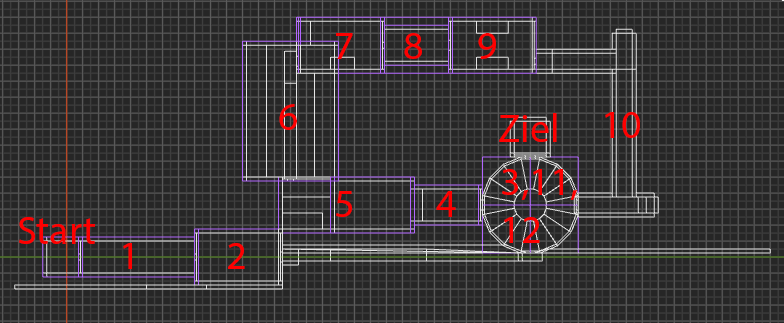
\includegraphics[width=0.9\linewidth]{Assets/Map Layout.png}
    \caption{
        \textbf{Maplayout}
        Das ist die map, raum 3 und 12 sind der gleiche, weil es ein kreislauf ist und raum 11 ist genau gleich gross einfach darüber, deswegen sind sie auf der karte gleich gekennzeichnet. Das ist das Mapout schema aus Trenchbroom.
    }
    \label{fig:Map}
\end{figure}

\subsubsection{Überblick über den Kampfabschnitt} \label{sec:Kampfabschnitt}

Unser Kampfabschnitt besteht aus zwölf Räumen. Jeder Raum bildet einen Encounter, der aus mehreren Wellen besteht; Anzahl und Grösse der Wellen sind für jeden Raum speziell konfiguriert. Eine neue Welle erscheint erst, nachdem alle Gegner der vorherigen Welle besiegt wurden. Eine Welle kann zwischen 10 und 30 Gegner enthalten.

Pro Welle lässt sich zudem festlegen, wie viele Gegner gleichzeitig im Raum sein dürfen (Abschnitt~\ref{sec:V2}). Stirbt ein Gegner, rückt ein weiterer nach. Die Reihenfolge, in der die Gegner erscheinen, ist im Voraus festgelegt. Jede Welle besteht aus einem Teil fest platzierter und einem Teil zufällig erscheinender Gegner (Abschnitt~\ref{sec:V5}). Nachdem alle Wellen eines Raumes besiegt wurden, öffnet sich genau eine Tür, durch die der Spieler weitergehen kann.

Tabelle~\ref{tab:Raeume} zeigt den Aufbau der einzelnen Räume; die Raumtypen werden in Abschnitt~\ref{sec:V6} erläutert.

\begin{table}[H]
    \centering
    \small
    \renewcommand{\arraystretch}{1.3}
    \begin{tabular}{|>{\raggedright\arraybackslash}p{0.9cm}|>{\raggedright\arraybackslash}p{1.6cm}|>{\raggedright\arraybackslash}p{1.1cm}|>{\raggedright\arraybackslash}p{5.5cm}|>{\raggedright\arraybackslash}p{3.6cm}|}
        \hline
        \textbf{Raum} & \textbf{Raumtyp} & \textbf{Wellen} & \textbf{Ablauf} & \textbf{Funktion} \\
        \hline
        1 & Intimate & 2 & Welle 1: ein Soldier. Welle 2: fünf Soldiers, höchstens zwei gleichzeitig. & Einführung des Soldiers; Spiel erklären \\
        \hline
        2 & Intimate & 2 & Welle 1: ein Archer. Welle 2: fünf Archer, höchstens zwei gleichzeitig. & Einführung des Archers \\
        \hline
        3 & Prospect & 3 & Pro Welle insgesamt etwa 10--15 Gegner, gemischt. & Erstmals gemischte Gegnertypen; Formationen und Dilemma (V3) werden vorgestellt \\
        \hline
        4 & Narrow & 3 & Welle 1: ein einzelner Soldier mit Überraschungsangriff. Welle 2: der Heavy Soldier alleine. Welle 3: Heavy Soldier in Kombination mit dem Archer. & Einführung des Heavy Soldiers; erste Plattform (Box), auf der man sich vor den Gegnern ausruhen kann \\
        \hline
        5 & Prospect & 2 & Welle 1: Archer, Soldier, Heavy Soldier, Welle 2: Archer, Soldier & Üben des gelernten und neue hindernisformation. \\
        \hline
        6 & Prospect & 3 & \textcolor{red}{[ergänzen]} & Einführung des Heavy Archers; Brücke als neues Hindernis \\
        \hline
        7 & Intimate & 3 & \textcolor{red}{[ergänzen]} & Einführung des Chain Archers \\
        \hline
        8 & Narrow & 3 & \textcolor{red}{[ergänzen]} & \textcolor{red}{[ergänzen]} \\
        \hline
        9 & Intimate & 2 & \textcolor{red}{[ergänzen]} & \textcolor{red}{[ergänzen]} \\
        \hline
        10 & Narrow & 3 & \textcolor{red}{[ergänzen]} & \textcolor{red}{[ergänzen]} \\
        \hline
        11 & Prospect & 1 & \textcolor{red}{[ergänzen]} & \textcolor{red}{[ergänzen]} \\
        \hline
        12 & Prospect & 2 & \textcolor{red}{[ergänzen]} & \textcolor{red}{[ergänzen]} \\
        \hline
    \end{tabular}
    \caption{Aufbau der Räume des Kampfabschnitts}
    \label{tab:Raeume}
\end{table}

\begin{itemize}[leftmargin=1.5cm]
    \item \textcolor{red}{Räume 5--12 in der Tabelle ergänzen (Raumtypen aus V6 und Einführungen aus V8 sind schon eingetragen).}
    \item \textcolor{red}{Widerspruch: \enquote{eine Welle kann zwischen 10 und 30 Gegner enthalten}, in Raum 1 und 2 haben die Wellen aber 1 bzw.\ 5 Gegner. Spannweite anpassen.}
    \item \textcolor{red}{Raumnummerierung prüfen: Im Playtest erwähnt TP2 \enquote{Raum 7.5}. Wie passt das zu den zwölf Räumen?}
    \item \textcolor{red}{Start und Ende des Kampfabschnitts kurz beschreiben.}
    \item \textcolor{red}{Molekül- oder Bubble-Diagramm des eigenen Kampfabschnitts (Methode aus Abschnitt~\ref{sec:Raumtypologien} und~\ref{sec:Prototyping} anwenden) sowie Draufsicht/Greybox-Screenshot.}
    \item \textcolor{red}{Vorgehen: Planung, Greybox (Trenchbroom), Iterationen; verworfene Varianten und Gründe.}
    \item \textcolor{red}{Umsetzung in Godot nur kurz (Szenenaufbau, Spawner/Wellensystem); Details mit Verweis auf die technische Dokumentation.}
    \item \textcolor{red}{Der Absatz zur Spannungskurve ist nach V7 verschoben.}
\end{itemize}

\subsubsection{V5: Lesbare Platzierung, dynamisches Verhalten} \label{sec:V5}

\paragraph{Vorschlag und Herleitung}
Gegner sollen zu Beginn lesbar und teils symmetrisch platziert sein, sich danach aber dynamisch verhalten, etwa den Spieler umzingeln. Der Nutzen betrifft Spielfluss und Spielgefühl: Die Anfangsaufstellung gibt Überblick, das anschliessende Verhalten hält den Kampf unter Druck und unvorhersehbar. Der Vorschlag verbindet die durchdachte, manuelle Platzierung aus \game{NieR: Automata} (Frage~A3) mit dem dynamischen Verhalten aus \game{Ninja Gaiden} (Frage~D3, Abschnitt~\ref{sec:Vergleich}) und stützt sich auf die Prinzipien der Lesbarkeit und der Gegner als raumbildende Elemente (Abschnitt~\ref{sec:Encounter}).

\paragraph{Umsetzung im Prototyp}
Besonders die erste Aufstellung der Gegner zu Beginn einer Welle haben wir oft manuell festgelegt, um eine Symmetrie in die Platzierung zu bringen. Die meisten Soldiers erscheinen dagegen zufällig, da sie sich bewegen können und ihre Startposition während des Kampfgeschehens deshalb keine allzu grosse Rolle spielt. Die Archers platzieren wir manuell, eher an den Rändern der Räume oder auf Hindernissen (Abschnitt~\ref{sec:V6}). Dadurch befinden sich oft Soldiers zwischen dem Spieler und den Archers, was das Dilemma aus Abschnitt~\ref{sec:V3} verstärkt.

Von ausserhalb des Raumes ist die erste Aufstellung allerdings nicht sichtbar, da die Gegner erst erscheinen, nachdem der Spieler den Raum betreten hat. Einen Eindruck der Raumgeometrie kann sich der Spieler jedoch schon vorher verschaffen.

Nach der Anfangsaufstellung verhalten sich die Gegner dynamisch: Gegner, die gerade nicht angreifen, halten Abstand zum Spieler und umkreisen ihn (Abschnitt~\ref{sec:V2}).

\begin{itemize}[leftmargin=1.5cm]
    \item \textcolor{red}{Klären: Bezieht sich \enquote{die meisten Soldiers erscheinen zufällig} auf die nachrückenden Gegner oder auch auf die erste Aufstellung? Sonst widerspricht es dem ersten Satz.}
    \item \textcolor{red}{Lesbarkeit: Wenn die Gegner erst nach dem Eintreten erscheinen, wie bekommt der Spieler trotzdem den Überblick (Spawn-Effekt, kurze Verzögerung, Symmetrie)? Ein Satz dazu stärkt V5.}
    \item \textcolor{red}{Abbildung mit eingezeichneten Spawnpunkten (z.\,B. Raum 3).}
\end{itemize}

\paragraph{Überprüfbarkeit}
\begin{itemize}[leftmargin=1.5cm]
    \item \textcolor{red}{Szene/Datei bzw. Verweis auf die technische Dokumentation.}
    \item \textcolor{red}{Playtest-Indikatoren: Q5, B6.}
\end{itemize}

\subsubsection{V6: Der Raum als Druckmittel} \label{sec:V6}

\paragraph{Vorschlag und Herleitung}
Die Grösse des Kampfraums soll gezielt zwischen Enge und Weite wechseln. Der Nutzen liegt in der Schwierigkeit, da ein enger Raum den Spieler zu methodischerem Spiel zwingt, während ein weiter Raum ihm taktische Distanz erlaubt. Vorbild ist die gezielte Raumverengung in \game{Ninja Gaiden} (Frage~M3), theoretisch untermauert durch die räumlichen Typologien Narrow und Prospect Space (Abschnitt~\ref{sec:Raumtypologien}).

\paragraph{Umsetzung im Prototyp}
In unserem Spiel gibt es eine Mischung aus den drei Raumtypen Narrow, Intimate und Prospect Space (Abschnitt~\ref{sec:Raumtypologien}). Jeder dieser Typen hat für den Spieler Vor- und Nachteile; Tabelle~\ref{tab:Raeume} zeigt die Zuordnung aller Räume.

\textbf{Intimate Spaces} sind Räume, in denen der Spieler genug Platz hat, sich zu bewegen und sein komplettes Moveset auszunutzen. In diesen Räumen ist der Spieler am stärksten im Vorteil. Nur vier unserer Räume fallen in diese Kategorie, nämlich die Räume 1, 2, 7 und 9. Die Räume 1 und 2 sind Intimate Spaces, weil hier die Kampfmechaniken beigebracht und die ersten Gegner vorgestellt werden; die Räume 7 und 9 sind es aufgrund der Spannungskurve.

\textbf{Narrow Spaces} sind, wie der Name sagt, enge Räume, in denen sich das Moveset des Spielers nicht vollständig entfalten kann. Davon haben wir drei, nämlich die Räume 4, 8 und 10. In Narrow Spaces sind eher die Nahkämpfer im Vorteil. Da unser Spiel besonders auf aggressive und schnelle Action ausgelegt ist, ergibt es wenig Sinn, viele enge Räume einzubauen, in denen man eher genau, taktisch und zurückhaltend spielen muss. Dennoch tragen sie zur Spannungskurve bei, weshalb wir einige davon haben.

\textbf{Prospect Spaces} sind die restlichen Räume 3, 5, 6, 11 und 12. Sie zeichnen sich dadurch aus, dass sie riesig sind und mehr als genug Platz bieten, um das Moveset des Spielers zu unterstützen. Sie sind sogar so gross, dass sie den Spieler verwundbar machen: Hier ist er den Archers eher unterlegen, da diese aus der Ferne angreifen können.

Die Räume einer Kategorie sind allerdings nicht zwangsläufig gleich gross. Ausschlaggebend für die Einordnung ist, wie gut sich der Spieler in einem Raum bewegen kann, und das hängt neben der Grösse von weiteren Variablen ab, vor allem von der Anzahl und den Typen der Gegner. So kann ein Raum riesig, aber dennoch ein Intimate und kein Prospect Space sein, weil in ihm nur wenige Gegner gleichzeitig erscheinen oder eher wenige Archers vorkommen.

In den Räumen befinden sich zudem Hindernisse, vor allem Boxen bzw.\ Container und in Raum~6 eine Brücke. Auf diesen erscheinen meistens die Archers, was es dem Spieler erschwert, an sie heranzukommen, und den Archers einen guten Überblick verschafft. Gleichzeitig können die Hindernisse dem Spieler als Deckung dienen. Der Spieler kann auch auf eine Box steigen, um sich zu heilen, da die Soldiers nicht springen können.

\begin{itemize}[leftmargin=1.5cm]
    \item \textcolor{red}{Eure Einteilung weicht von Totten ab: Dort werden die Typen über die Raumwirkung/Grösse definiert, bei euch über die Bewegungsfreiheit des Spielers inklusive Gegneranzahl und -typen. Das ist legitim, sollte aber ausdrücklich als eigene Anpassung von Tottens Typologie bezeichnet werden.}
    \item \textcolor{red}{\enquote{aufgrund der Spannungskurve} (Räume 7 und 9) kurz erklären, z.\,B. als Entlastung nach einem Narrow Space (Raum 8)?}
    \item \textcolor{red}{Optional: Grundriss oder Screenshot je Raumtyp (\enquote{Eigene Abbildung}).}
\end{itemize}

\paragraph{Überprüfbarkeit}
\begin{itemize}[leftmargin=1.5cm]
    \item \textcolor{red}{Szene/Datei bzw. Verweis auf die technische Dokumentation.}
    \item \textcolor{red}{Playtest-Indikatoren: Q6, B7.}
\end{itemize}

\subsubsection{V7: Wellenstruktur mit Erholungsphasen} \label{sec:V7}

\paragraph{Vorschlag und Herleitung}
Der Kampfabschnitt soll in Wellen mit kontrollierter Eskalation und kurzen Erholungsphasen dazwischen aufgebaut sein. Der Nutzen betrifft den Spielfluss, indem sich Anspannung und Entlastung abwechseln und die Schwierigkeit planbar ansteigt. Beide Referenzspiele nutzen dieses Muster (Frage~D1 in \game{Ninja Gaiden}, Frage~A4 in \game{NieR: Automata}), das der Recherche als Rollercoaster-Pacing bekannt ist (Abschnitt~\ref{sec:Pacing}).

\paragraph{Umsetzung im Prototyp}
Wie die Wellen technisch funktionieren, ist in Abschnitt~\ref{sec:Kampfabschnitt} beschrieben. Unser Prototyp weist eine zweifache Wellenstruktur auf: zum einen von Raum zu Raum und zum anderen, offensichtlicher, von Welle zu Welle. Die Spannungskurve entwickelt sich entsprechend auf beiden Ebenen: In den meisten Räumen gibt es einfachere und schwerere Wellen, und es gibt Räume, die insgesamt schwerer oder einfacher sind.

Die Schwierigkeit steigt mit der Anzahl der Gegner und mit der Einführung neuer Gegnertypen (Abschnitt~\ref{sec:V8}). Besonders deren Kombination im Raum erhöht die Schwierigkeit.

Am Ende eines Raumes kann sich der Spieler immer so lange erholen, wie er möchte, bevor er in den nächsten Raum geht. Zwischen den Wellen gibt es dagegen nicht viel Erholungszeit, denn die nächste Welle erscheint direkt, nachdem alle Gegner der vorherigen besiegt wurden. Abgesehen von leichteren Wellen besteht die einzige Erholungsmöglichkeit hier darin, den letzten Gegner am Leben zu lassen und sich so selbst Erholungszeit zu verschaffen. Innerhalb eines Raumes kann man sich zudem auf den Boxen ausruhen, sofern man diese von Gegnern befreit hat (Abschnitt~\ref{sec:V6}).

\begin{itemize}[leftmargin=1.5cm]
    \item \textcolor{red}{Der Vorschlag verlangt \enquote{kurze Erholungsphasen} zwischen den Wellen, umgesetzt gibt es kaum welche. Bewusst so? Kurz begründen und in Kapitel~\ref{sec:Evaluation} diskutieren (TP2 spricht von \enquote{überlappenden Wellen} und schwer zu findenden Heilpausen).}
    \item \textcolor{red}{\enquote{Den letzten Gegner leben lassen}: beabsichtigt oder von euch/Testpersonen entdeckt? Klarstellen.}
    \item \textcolor{red}{Optional: Diagramm der geplanten Spannungskurve über die Räume 1--12 (mit Raumtypen). Das macht die Eskalation überprüfbar.}
\end{itemize}

\paragraph{Überprüfbarkeit}
\begin{itemize}[leftmargin=1.5cm]
    \item \textcolor{red}{Szene/Datei bzw. Verweis auf die technische Dokumentation.}
    \item \textcolor{red}{Playtest-Indikatoren: Q7, B8.}
\end{itemize}

\subsubsection{V8: Gestaffelte Einführung neuer Gegner} \label{sec:V8}

\paragraph{Vorschlag und Herleitung}
Jeder neue Gegnertyp soll zuerst isoliert auftreten und erst danach mit anderen kombiniert werden. Der Nutzen betrifft Spielfluss und Schwierigkeit, weil der Spieler einen Gegner in Ruhe verstehen kann, bevor die Kombination ihn fordert. Grundlage ist das Scaffolding-Prinzip (Abschnitt~\ref{sec:Scaffolding}) sowie die entsprechende Struktur in \game{NieR: Automata} (Frage~D1).

\paragraph{Umsetzung im Prototyp}
Wie Tabelle~\ref{tab:Raeume} zeigt, werden unsere fünf Gegnertypen in den Räumen 1, 2, 4, 6 und 7 vorgestellt. In den Räumen 1 und 2 wollen wir die Basisgegner vorstellen und gleichzeitig das Spiel erklären. Sobald sich der Spieler an das Neue gewöhnt hat, folgt ein neuer Gegnertyp. Gleichzeitig wollten wir alle Gegner früh genug vorgestellt haben, um anschliessend verschiedene Kombinationen mit ihnen ausprobieren zu können.

Der Heavy Soldier wurde im ersten Narrow Space (Raum~4) eingeführt, um ihn noch bedrohlicher wirken zu lassen. Der Heavy Archer wurde hingegen in einem Prospect Space (Raum~6) vorgestellt, da er sich besonders in grossen Räumen als bedrohlich erweist. Der Chain Archer wurde in einem Intimate Space (Raum~7) vorgestellt, um dem Soldier im Raumtyp, in dem der Spieler die grössten Vorteile hat, etwas den Platz streitig zu machen.

Damit halten wir uns an unsere Recherche, nach der pro Raum etwa eine neue Mechanik eingeführt werden sollte, um den Spieler nicht zu stark zu belasten und das Spiel dennoch unterhaltsam zu gestalten (Abschnitt~\ref{sec:Scaffolding}).

\begin{itemize}[leftmargin=1.5cm]
    \item \textcolor{red}{Korrigiert: In eurem Text stand \enquote{Der Heavy Archer wurde im ersten Narrow Raum eingeführt}. Laut Tabelle ist das der Heavy Soldier in Raum~4 -- bitte prüfen.}
    \item \textcolor{red}{\enquote{um dem Soldier etwas den Platz streitig zu machen}: gemeint ist wohl \emph{dem Spieler}? Prüfen.}
    \item \textcolor{red}{Die Recherche spricht von einer neuen Mechanik \emph{pro Level}, ihr setzt das \emph{pro Raum} um. Diese Anpassung in einem Halbsatz begründen.}
    \item \textcolor{red}{Braiding: kurz nennen, wo die neuen Typen erstmals mit anderen kombiniert werden (z.\,B. Raum~3, Raum~4 Heavy Soldier + Archer).}
\end{itemize}

\paragraph{Überprüfbarkeit}
\begin{itemize}[leftmargin=1.5cm]
    \item \textcolor{red}{Szene/Datei bzw. Verweis auf die technische Dokumentation.}
    \item \textcolor{red}{Playtest-Indikatoren: Q8, B9.}
\end{itemize}

\end{document}
